\documentclass[paper=letter,11pt]{scrartcl}

\KOMAoptions{headinclude=true, footinclude=false}
\KOMAoptions{DIV=14, BCOR=5mm}
\KOMAoptions{numbers=noendperiod}
\KOMAoptions{parskip=half}
\addtokomafont{disposition}{\rmfamily}
\addtokomafont{part}{\LARGE}
\addtokomafont{descriptionlabel}{\rmfamily}
%\setkomafont{pageheadfoot}{\normalsize\sffamily}
\setkomafont{pagehead}{\normalsize\rmfamily}
%\setkomafont{publishers}{\normalsize\rmfamily}
\setkomafont{caption}{\normalfont\small}
\setcapindent{0pt}
\deffootnote[1em]{1em}{1em}{\textsuperscript{\thefootnotemark}\ }


\usepackage{amsmath}
\usepackage[varg]{txfonts}
\usepackage[T1]{fontenc}
\usepackage{graphicx}
\usepackage{xcolor}
\usepackage[american]{babel}
% hyperref is needed in many places, so include it here
\usepackage{hyperref}

\usepackage{xspace}
\usepackage{multirow}
\usepackage{float}


\usepackage{braket}
\usepackage{bbm}
\usepackage{relsize}
\usepackage{tcolorbox}

\def\ketY{\ensuremath{\ket {\Psi}}}
\def\iGeV{\ensuremath{\textrm{GeV}^{-1}}}
%\def\mp{\ensuremath{m_{\textrm{proton}}}}
\def\rp{\ensuremath{r_{\textrm{proton}}}}
\def\me{\ensuremath{m_{\textrm{electron}}}}
\def\aG{\ensuremath{\alpha_G}}
\def\rAtom{\ensuremath{r_{\textrm{atom}}}}
\def\rNucl{\ensuremath{r_{\textrm{nucleus}}}}
\def\GN{\ensuremath{\textrm{G}_\textrm{N}}}
\def\ketX{\ensuremath{\ket{\vec{x}}}}
\def\ve{\ensuremath{\vec{\epsilon}}}


\def\ABCDMatrix{\ensuremath{\begin{pmatrix} A &  B  \\ C  & D \end{pmatrix}}}
\def\xyprime{\ensuremath{\begin{pmatrix} x' \\ y' \end{pmatrix}}}
\def\xyprimeT{\ensuremath{\begin{pmatrix} x' &  y' \end{pmatrix}}}
\def\xy{\ensuremath{\begin{pmatrix} x \\ y \end{pmatrix}}}
\def\xyT{\ensuremath{\begin{pmatrix} x & y \end{pmatrix}}}

\def\IMatrix{\ensuremath{\begin{pmatrix} 0 &  1  \\ -1  & 0 \end{pmatrix}}}
\def\IBoostMatrix{\ensuremath{\begin{pmatrix} 0 &  1  \\ 1  & 0 \end{pmatrix}}}
\def\JThree{\ensuremath{\begin{pmatrix}    0 & -i & 0  \\ i & 0  & 0 \\ 0 & 0 & 0 \end{pmatrix}}} 
\def\JTwo{\ensuremath{\begin{bmatrix}    0 & 0 & -i  \\ 0 & 0  & 0 \\ i & 0 & 0 \end{bmatrix}}}
\def\JOne{\ensuremath{\begin{bmatrix}    0 & 0 & 0  \\ 0 & 0  & -i \\ 0 & i & 0 \end{bmatrix}}}
\def\etamn{\ensuremath{\eta_{\mu\nu}}}
\def\Lmn{\ensuremath{\Lambda^\mu_\nu}}
\def\dmn{\ensuremath{\delta^\mu_\nu}}
\def\wmn{\ensuremath{\omega^\mu_\nu}}
\def\be{\begin{equation*}}
\def\ee{\end{equation*}}
\def\bea{\begin{eqnarray*}}
\def\eea{\end{eqnarray*}}
\def\bi{\begin{itemize}}
\def\ei{\end{itemize}}
\def\fmn{\ensuremath{F_{\mu\nu}}}
\def\fMN{\ensuremath{F^{\mu\nu}}}
\def\bc{\begin{center}}
\def\ec{\end{center}}
\def\nus{$\nu$s}

\def\adagger{\ensuremath{a_{p\sigma}^\dagger}}
\def\lineacross{\noindent\rule{\textwidth}{1pt}}

\newcommand{\multiline}[1] {
\begin{tabular} {|l}
#1
\end{tabular}
}

\newcommand{\multilineNoLine}[1] {
\begin{tabular} {l}
#1
\end{tabular}
}



\newcommand{\lineTwo}[2] {
\begin{tabular} {|l}
#1 \\
#2
\end{tabular}
}

\newcommand{\rmt}[1] {
\textrm{#1}
}


%
% Units
%
\def\m{\ensuremath{\rmt{m}}}
\def\GeV{\ensuremath{\rmt{GeV}}}
\def\pt{\ensuremath{p_\rmt{T}}}


\def\parity{\ensuremath{\mathcal{P}}}

\usepackage{cancel}
\usepackage{ mathrsfs }
\def\bigL{\ensuremath{\mathscr{L}}}

\usepackage{ dsfont }



\usepackage{fancyhdr}
\fancyhf{}

%\documentclass[margin,line]{res}
\usepackage{braket}
\usepackage{bbm}
\usepackage{relsize}

\def\ketY{\ensuremath{\ket {\Psi}}}
\def\iGeV{\ensuremath{\textrm{GeV}^{-1}}}


\def\ABCDMatrix{\ensuremath{\begin{pmatrix} A &  B  \\ C  & D \end{pmatrix}}}
\def\xyprime{\ensuremath{\begin{pmatrix} x' \\ y' \end{pmatrix}}}
\def\xyprimeT{\ensuremath{\begin{pmatrix} x' &  y' \end{pmatrix}}}
\def\xy{\ensuremath{\begin{pmatrix} x \\ y \end{pmatrix}}}
\def\xyT{\ensuremath{\begin{pmatrix} x & y \end{pmatrix}}}

\def\IMatrix{\ensuremath{\begin{pmatrix} 0 &  1  \\ -1  & 0 \end{pmatrix}}}
\def\IBoostMatrix{\ensuremath{\begin{pmatrix} 0 &  1  \\ 1  & 0 \end{pmatrix}}}
\def\JThree{\ensuremath{\begin{pmatrix}    0 & -i & 0  \\ i & 0  & 0 \\ 0 & 0 & 0 \end{pmatrix}}} 
\def\JTwo{\ensuremath{\begin{bmatrix}    0 & 0 & -i  \\ 0 & 0  & 0 \\ i & 0 & 0 \end{bmatrix}}}
\def\JOne{\ensuremath{\begin{bmatrix}    0 & 0 & 0  \\ 0 & 0  & -i \\ 0 & i & 0 \end{bmatrix}}}
\def\etamn{\ensuremath{\eta_{\mu\nu}}}
\def\Lmn{\ensuremath{\Lambda^\mu_\nu}}
\def\dmn{\ensuremath{\delta^\mu_\nu}}
\def\wmn{\ensuremath{\omega^\mu_\nu}}
\def\be{\begin{equation*}}
\def\ee{\end{equation*}}
\def\bc{\begin{center}}
\def\ec{\end{center}}
\def\nus{$\nu$s}
\def\nue{\ensuremath{\nu_e}}
\def\numu{\ensuremath{\nu_\mu}}
\def\nutau{\ensuremath{\nu_\tau}}
\def\nualpha{\ensuremath{\nu_\alpha}}
\def\nuone{\ensuremath{\nu_1}}
\def\nutwo{\ensuremath{\nu_2}}
\def\nuthree{\ensuremath{\nu_3}}
%\def\xMu{\ensuremath{x^\mu}

\usepackage{fancyhdr}

\fancyhf{}
\lhead{\Large 33-444} % \hfill Introduction to Particle Physics \hfill Spring 2019}
\chead{\Large Introduction to Particle Physics} % \hfill Spring 2019}
\rhead{\Large Spring 2019} % \hfill Introduction to Particle Physics \hfill Spring 2019}

\begin{document}
\thispagestyle{fancy}

\begin{center}
{\huge \textbf{Lecture 34}}
\end{center}

{\fontsize{14}{16}\selectfont

\textbf{\underline{OK left off discussing atmospheric \nus}} 

Saw that there are two robust predictions that you can measure:
\begin{itemize}
\item[-]muon vs electron ratio and
\item[-]top vs down ratio. 
\end{itemize}

Expect the same amount from above and from below.

So that's what people know about atmospheric \nus. 

The experiments that measured atmospheric \nus\ where giant water tanks.

Kamiokande - Name Kamioka place / nde - ``nucleon decay experiment. ``

Built to look for proton decay, but atmospheric \nus\ where a background one you cant get rid of. 

When you measure the flux from above and below turns out the answer is not one: 1/2.

They could actually do better. 
Tell muons from electrons.
These plots show log/high energy electrons and muons separately. 
\clearpage

\begin{figure}[h!]
\centering
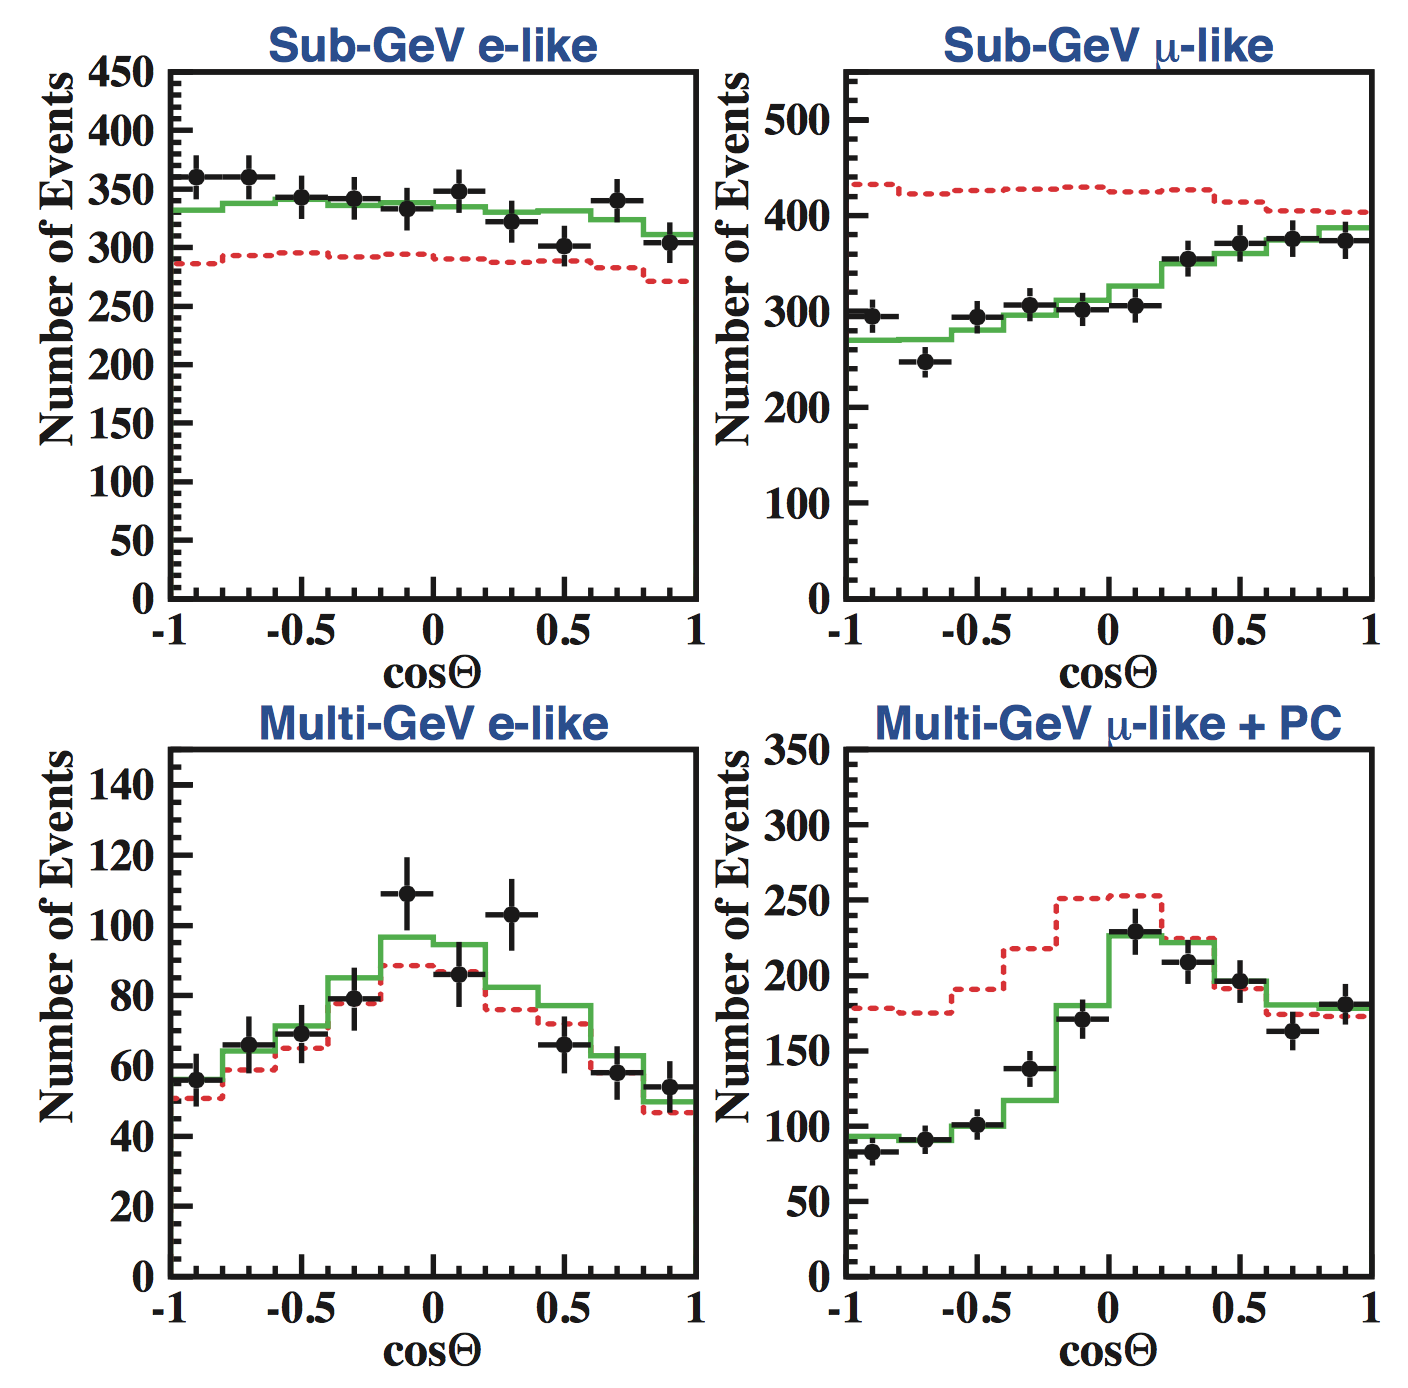
\includegraphics[width=1.0\textwidth]{./sk.png}
\end{figure}
\clearpage

Very interesting resultsx.
Points are the observations, solid line is the prediction.
Notice a few things; 
\begin{itemize}
\item[-] For the electrons everything works more or less OK, 
\item[-] For the muons it doesn work well at all.
\item[-] \nus coming from above work OK, 
\item[-] \nus coming from below don't work well. (Missing about half of them.)
\end{itemize}
You have an effect that says you don't understand what the muon \nus are doing and that effect depends on the energy and how far they are propagating.


Very exciting result. 
Because you're sure the measurements are correct. 
Observable is robust. 
Implies that the \nus\ are doing something. 
And whatever they are doing depends on the energy and the baseline (how much they have traveled)

Why is this important ? need a hypothesis for what is going on. 
Maybe the \nus\ are being absorbed ? 
\nus\ that go through the earth are getting absorbed by the earth. 
Know Cant be true,  cross section would have to be too high. 

What else could be going on?
\nus\ decaying /changing flavour
Only looking for muon and electron \nus, so if they were converting into $\tau$s, this could explain all this data.
Only massive particles know about time. 
What ever they are doing 
If \nus can tell time ==> \nus have mass. 
OR Lorentz invariance is wrong. 

So that's where we were. 
Bottom line \nus change flavour as a function of E and distance. 

\noindent\rule{\textwidth}{1pt}

\textbf{Mass-induced flavour oscillations.}

What happens if the \nus\ have mass ?

\be
\nu_1 \textrm{ with } m_1
\ee
\be
\nu_2 \textrm{ with } m_2
\ee
\be
\nu_3 \textrm{ with } m_3
\ee

If you raise the hypothesis that \nus\ have mass, then there are \nus\ states that you can label with different masses.

We also have \nue, \numu\ and \nutau\ these are the interaction eigenstatss the \nus\ you produce when you have a weak interaction. 

The question is then which one of these is the \nue, \numu\ and \nutau ?

The answer is it doesn't have to be any of them, know for sure is that the \nue\ is a linear combination of \nus\ with a well-defined bass
\be
\nue = U_ei \nu_i
\ee
same for mus and taus. 
\be
\numu = U_{\mu\ i} \nu_i
\ee
\be
\nutau = U_{\tau\ i} \nu_i
\ee
also know that the \nue, \numu\ and \nutau or orthogonal to one another (ie: they are different states) 

These can then be organised into a unitary matrix. 
\be
\nualpha = U_{\alpha\ i} \nu_i
\ee
where, $\alpha = e, \mu, \tau$ and $i = 1,2,3$.

$U_{\alpha i}$ is Unitary mixing matrix
We will see, just by raising this hypothesis you can explain all the data.

\noindent\rule{\textwidth}{1pt}
\textbf{Parallel in Quark Sector}

Actually similar thing happens in the quark sector, we haven't talked about this yet, but its true.

Have do identify who are the ``real particles''. 
Meaning what are the eigenstates of the free Hamiltonian.

In the quark section that's the 

u c t \\
d s b

In the lepton sector we choose that to be 

$e\ \mu\ \tau$ \\
$\nuone\ \nutwo\ \nuthree $

There is no such thing as an \nue, doesn't exist. 

but the weak interactions couple to linear combinations of these real particles.  

$W \rightarrow t + b,s,b$ w/coupling $V_{CKM}$  $U_t,\alpha$

the same thing happens in the lepton sector:


$W \rightarrow e + \nuone,\nutwo,\nuthree$ w/coupling $U_e,i$

physics is the same,  the consequences turn out to be very different.  
Main reason is that the $\nu$ masses  are very small. 
Bc the masses are small (as well talk about in a second) you have a phenomena of $\nu$ oscillations.
Doesn't happen for quarks. 

\noindent\rule{\textwidth}{1pt}

\textbf{$\nu$ Oscillations}

OK lets set up this physics behind this idea.. 

What does it mean to be a particle with a well defined mass?
QM point-of-view, eigenstates of free particle Hamiltonian. 

\be
\ket{\nuone} =  e^{-iE_1t} \ket{\nuone}
\ee

this is what ti means to be a $\nu$ with a well-defined mass.

Now, what happens if you don't have one of these, but a linear superposition  ?

Lets say you have the \nue\ and, to make life easy, lets pretend that we only have 2 \nus. 

Now \nue\ will be a linear combination of \nuone\ and \nutwo. 
\be
\ket{\nue} = \cos\theta \ket{\nuone} + \sin\theta \ket{\nutwo}
\ee
For completeness, can also write \numu, which is also a linear combination of \nuone\ and \nutwo, but it is a orthogonal to \nue.
\be
\ket{\numu} = -\sin\theta \ket{\nuone} + \cos\theta \ket{\nutwo}
\ee


Some obvious things, we know $\cos\theta$ and $\sin\theta$ are some coefficients that we don't know, but we know the sum of squares is 1. 
That's why we write it like an angle.
(Can work this out from  $\braket{\nue | \nue}  = 1$ and $\braket{\nue | \numu}  = 0$)
That's why are allowed to paramaterize things this way

How do these states evolve as a function of time?
\be
\ket{\nue(t)} = \cos\theta e^{-iE_1t} \ket{\nuone} + \sin\theta e^{-iE_2t}\ket{\nutwo}
\ee
This is the heart of what $\nu$ oscillations are all about. 
Because these phases are different, what you get is no longer proportional to the \nue\ state.
Or in fancier words, \nue\ is not an eigenstate of the free Hamiltonian.

Now this is very very simple physics. 
Literally a 2 level system that you learned in undergraduate QM.


Remember everything is going to be relativistic. 
\nus\ are going to be propagating plane waves. 

Relativistic version 

\be
\ket{\nue(\vec{x},t)} = \cos\theta e^{-ip_1^\mu x_\mu} \ket{\nuone} + \sin\theta e^{-ip_2^\mu x_\mu}\ket{\nutwo}
\ee
where x is the $(t,\vec{x})$ four vector. 

\noindent\rule{\textwidth}{1pt}

\textbf{Ultra relativistic approx. }

\be
t \sim L 
\ee
Phase factors very close to being zero, depend on difference between energy and momentum $(E_1 - p_1)$


Now let me calculate this difference in the following way,
\be
(E_1 - p_1)(E_1 + p_1) = m_1^2  \Rightarrow  (E_1 - p_1) = \frac{m_1^2}{2E} 
\ee
in the ultra relativistic approx $E \sim P$


\be
\ket{\nue(L)} = \cos\theta e^{-i \frac{m_1^2}{2E} L} \ket{\nuone} + \sin\theta e^{-i \frac{m_2^2}{2E} L} \ket{\nutwo}
\ee

OK, now lets calculate something...


Lets calculate the probability that this object here, when it hits something produces an electron. 

Which is just given by 
\be
\braket{\nue | \nue(L) } = \cos^2 \theta e^{-i \frac{m_1^2}{2E} L} + \sin^2\theta e^{-i \frac{m_2^2}{2E} L} 
\ee
is the amplitude for having an \nue\ be born somewhere, propagate some distance L and then be detected as an \nue.
So the probability is this thing squared:
\begin{eqnarray*}
\left|\braket{\nue | \nue(L) }\right|^2 &=& \left|\cos^2 \theta e^{-i \frac{m_1^2}{2E} L} + \sin^2\theta e^{-i \frac{m_2^2}{2E} L} \right|^2\\
       &=& \left|\cos^2 \theta+ \sin^2\theta e^{-i \frac{m_2^2 - m_1^2}{2E} L} \right|^2\\
       &=& \cos^4 \theta+ \sin^4\theta  + \cos^2\theta \sin^2 \theta 2 \cos \left( \frac{\Delta m^2 L}{2E} \right)
\end{eqnarray*}
where $\Delta m^2 = m_2^2 - m_1^2$.
Can simply this...
\begin{eqnarray*}
 &=& \left( \cos^2 \theta + \sin^2 \theta \right)^2  - 2 \cos^2 \theta \sin^2 \theta  + 2 \cos^2 \theta \sin^2 \theta \cos \left( \frac{\Delta m^2 L}{2E} \right) \\
 &=& 1 - 2 \cos^2 \theta \sin^2 \theta \left( 1  - \cos \left( \frac{\Delta m^2 L}{2E} \right) \right)
\end{eqnarray*}
Now use some  trig IDs...
\begin{eqnarray*}
 &=& 1 - 4 \sin^2 \theta \cos^2 \theta \sin^2 \left( \frac{\Delta m^2 L}{2E} \right)\\
 &=& 1 -  \sin^2 2\theta \sin^2 \left( \frac{\Delta m^2 L}{2E} \right)
\end{eqnarray*}

So what we learn at the end of the day is, if your born as \nue and you propagate a certain distance L, and you're detected as an \nue, the probability is given by,
\be 
P_{ee}(L) = 1 - \sin^2 2\theta \sin^2 \left( \frac{\Delta m^2 L}{2E} \right)
\ee 
Possible to be born as \nue\ and detected as \nue\ with less than 100\% probability!

}
\end{document}


